\section{矩阵}

\subsection{矩阵的逆}\label{thm:2.1}
\begin{theorem}
设$A$为$n$阶方阵,$A^*$为$A$的伴随矩阵,若$|A| \neq 0$,则$A$是一个非异阵,且
  \begin{equation}
  A^{-1}=\frac{1}{|A|}A^*.
\end{equation}

\end{theorem}

\begin{proof}
  \begin{equation*}
    AA^*=
    \begin{pmatrix}
      a_{11} & a_{12} & \cdots & a_{1n}\\
      a_{21} & a_{22} & \cdots & a_{2n}\\
      \vdots & \vdots & & \vdots\\
      a_{n1} & a_{n2} & \cdots & a_{nn}
    \end{pmatrix}
    \begin{pmatrix}
      A_{11} & A_{21} & \cdots & A_{n1}\\
      A_{12} & A_{22} & \cdots & A_{n2}\\
      \vdots & \vdots & & \vdots\\
      A_{1n} & A_{2n} & \cdots & A_{nn}
    \end{pmatrix}.
    \end{equation*}
    上式中两个矩阵乘积的第$(i,j)$元素为
    \begin{equation*}
      a_{i1}A_{j1}+a_{i2}A_{j2}+\cdots+a_{in}A_{jn}.
    \end{equation*}
    按照定理\eqref{thm:1-1}可知:
    当$i=j$时上式为$|A|$,当$i \neq j$时上式为零。因此
    \begin{equation*}
      AA^*=
      \begin{pmatrix}
        |A| & 0 & \cdots & 0\\
        0 & |A| & \cdots & 0\\
        \vdots & \vdots & \ddots & \vdots\\
        0 & 0 & \vdots & |A|
      \end{pmatrix}=|A|\cdot I_n.
    \end{equation*}
同理可证
\begin{equation*}
  A^*A=|A|\cdot I_n.
\end{equation*}
因为$|A|\neq 0$,由以上二式同除以$|A|$可以得到
\begin{equation*}
  A(\frac{1}{|A|}A^*)=(\frac{1}{|A|}A^*)A=I_n,
\end{equation*}
因此
\begin{equation*}
  A^{-1}=\frac{1}{|A|}A^*
\end{equation*}
A是非异阵.
\end{proof}

\subsection{\texorpdfstring{$Cauchy-Binet$}{\textit{Cauchy-Binet}}公式}

\begin{theorem}[$Cauchy-Binet$公式]\label{thm:Cauchy-Binet}
  设 $A=(a_{ij})$是$m \times n$矩阵,$B=(b_{ij})$是$n \times m$矩阵.
  $A\left(\begin{smallmatrix}i_1 & \cdots & i_s \\
      j_1 & \cdots & j_s \end{smallmatrix}\right)$
  表示$A$的一个$s$阶子式,它由$A$的第$i_1, \cdots, i_s$行与第
  $j_1, \cdots, j_s$列交点上的元素按原次序排列组成的行列式,
  同理可定义$B$的$s$阶子式.\par
  (1)若$m>n$,则必有$\left\vert AB \right\vert=0$;\par
  (2)若$m \le n$,则必有\par
  $|AB|= \sum\limits_{1 \le j_1<j_2<\cdots<j_m \le n}
  A\left(\begin{smallmatrix}
      1 & 2 & \cdots & m \\
      j_1 & j_2 & \cdots & j_m \end{smallmatrix}\right)
  B\left(\begin{smallmatrix}
      j_1 & j_2 & \cdots & j_m\\
      1 & 2 & \cdots & m \end{smallmatrix}\right)$

\end{theorem}

\begin{proof}
  令$C=\left(\begin{smallmatrix}
      A & O\\
      -I_n & B \end{smallmatrix}\right)$.
  用不同方法表示行列式$|C|$:

  首先, 对$C$进行第三类分块初等变换, 得到矩阵$M=\left(\begin{smallmatrix}
      O & AB\\
      -I_n & B \end{smallmatrix}\right)$, $M$可以改写为
  $M = \left(\begin{smallmatrix}
      I_m & A\\
      O & I_n \end{smallmatrix}\right)C$. 
  因此, $|M| = |C|$. 

  用Laplace定理来计算$\left\vert M \right\vert$, 
  由于$AB$占据$M$的前$m$行和第$n+1$至第$n+m$列, 
  $M$除$AB$外, 前$m$行的其余列都是$0$, 因此$|M|$按前$m$行展开得
  \begin{align*}
    |M| & =(-1)^{(n+1+n+2+\cdots+n+m)+(1+2+\cdots+m)}|-I_n||AB|\\
        & =(-1)^{nm+m(m+1)+n}|AB|
  \end{align*}
  
  上面第二个等式是因为$|-I_n|=(-1)^n$. 
  由于$m(m+1)$总是偶数, 可以去掉该式, 且$nm+n=n(m+1)$, 所以
  \begin{equation}\label{eq:5}
    |M|=(-1)^{n(m+1)}|AB|.
  \end{equation}  

  再计算$|C|$,用$Laplace$定理按前$m$行展开,分两种情况:

  若$m > n$,则$A$为瘦长型的矩阵,$B$为矮胖型矩阵,如图\ref{fig:1}所示:\\
  \begin{figure}[!ht]
   \begin{center}
  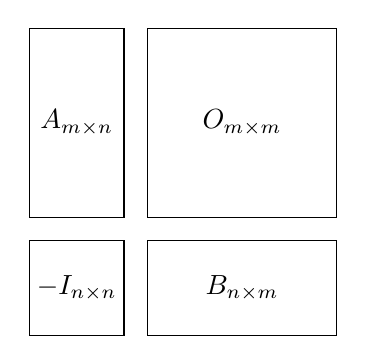
\begin{tikzpicture}[scale=0.3]
    \draw (0,0) rectangle (4,4); 
    \draw (5,5) rectangle (13,13);
    \draw (0,5) rectangle (4,13);
    \draw (5,0) rectangle (13,4);
    \node at (2,9) {$A_{m\times n}$};
    \node at (2,2) {$-I_{n\times n}$};
    \node at (9,2) {$B_{n\times m}$};
    \node at (9,9) {$O_{m\times m}$}; 
  \end{tikzpicture}
  \end{center}
  \caption{瘦长型矩阵$A$\label{fig:1}}
\end{figure}  前$m$行中任意一个$m$阶子式至少有一列全部为$0$,
即要从$O$中获取$m-n$列用于构建$m$阶子式,因此整个行列式的值为$0$,
即$|AB|=0$.

若$m \le n$,则$A$为矮胖型矩阵,$B$为瘦长型的矩阵,如图\ref{fig:2}所示:

  \begin{figure}[!ht]
   \begin{center}
  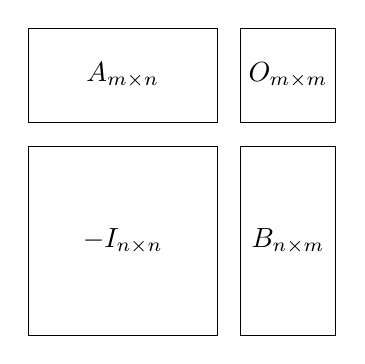
\begin{tikzpicture}[scale=0.3]
    \draw (0,0) rectangle (8,8);
    \draw (9,9) rectangle (13,13);
    \draw (0,9) rectangle (8,13);
    \draw (9,0) rectangle (13,8);
    \node at (4,11) {$A_{m\times n}$};
    \node at (4,4) {$-I_{n\times n}$};
    \node at (11,4) {$B_{n\times m}$};
    \node at (11,11) {$O_{m\times m}$}; 
  \end{tikzpicture}
  \end{center}
  \caption{矮胖型矩阵$A$\label{fig:2}}
\end{figure}
由Laplace定理得
\begin{equation}\label{eq:1}
  |C|= \sum\limits_{1<=j_1<j_2<\cdots<j_m<=n}
  A\left(\begin{smallmatrix}
      1 & 2 & \cdots & m \\
      j_1 & j_2 & \cdots & j_m \end{smallmatrix}\right)
  \hat C\left(\begin{smallmatrix}
      1 & 2 & \cdots & m \\
      j_1 & j_2 & \cdots & j_m
    \end{smallmatrix}\right),
\end{equation}
其中,$\hat C\left(\begin{smallmatrix}
      1 & 2 & \cdots & m \\
      j_1 & j_2 & \cdots & j_m
      \end{smallmatrix}\right)$是$A\left(\begin{smallmatrix}
      1 & 2 & \cdots & m \\
      j_1 & j_2 & \cdots & j_m \end{smallmatrix}\right)$
  在矩阵$C$中的代数余子式.显然,
  \begin{equation}\label{eq:2}
    \hat C\left(\begin{smallmatrix}
      1 & 2 & \cdots & m \\
      j_1 & j_2 & \cdots & j_m
    \end{smallmatrix}\right)=(-1)^{\frac{1}{2}m(m+1)+(j_1+j_2+\cdots+j_m)}%
  |-e_{i_1},-e_{i_2},\cdots,-e_{i_{n-m}},B|,
  \end{equation}
  其中$i_1,i_2,\cdots,i_{n-m}$是$C$中前$n$列去掉$j_1,j_2,\cdots,j_m$列后
  余下的列序数.$e_{i_1},e_{i_2},\\\cdots,e_{i_{n-m}}$是相应的$n$维标准单位列
  向量.$\hat C$除了包含全部$B$,还需要从$-I_n$中获取$n-m$个列.记
  \[
    |N|=|-e_{i_1},-e_{i_2},\cdots,-e_{i_{n-m}},B|,
  \]

  下面计算$|N|$.$|N|$用$Laplace$定理按前$n-m$列展开,只有一个子式非零,
  其值等于$|-I_{n-m}|=(-1)^{n-m}$.这个子式的余子式为$B\left(\begin{smallmatrix}
      j_1 & j_2 & \cdots & j_m\\
      1 & 2 & \cdots & m \end{smallmatrix}\right)$.因此,
  \begin{equation}\label{eq:3}
    |N| = (-1)^{(n-m)+(i_1+i_2+\cdots+i_{n-m})+(1+2+\cdots+n-m)}%
    B\left(\begin{smallmatrix}
      j_1 & j_2 & \cdots & j_m\\
      1 & 2 & \cdots & m \end{smallmatrix}\right).
  \end{equation}

  将\eqref{eq:3}式代入\eqref{eq:2}式,再将\eqref{eq:2}式代入\eqref{eq:1}式得
\begin{equation}\label{eq:4}
  |C|=\sum\limits_{1\le j_1<j_2<\cdots<j_m\le n}
  (-1)^{l}
  A\left(\begin{smallmatrix}
      1 & 2 & \cdots & m \\
      j_1 & j_2 & \cdots & j_m \end{smallmatrix}\right)
  B\left(\begin{smallmatrix}
      j_1 & j_2 & \cdots & j_m\\
      1 & 2 & \cdots & m \end{smallmatrix}\right)
\end{equation}

其中,$l=\frac{1}{2}m(m+1)+(j_1+j_2+\cdots+j_m)+(n-m)+(i_1+i_2+\cdots+i_{n-m})+
(1+2+\cdots+n-m)$.从图\eqref{fig:2}可知,$j_1+j_2+\cdots+j_m$是被选取到
$A\left(\begin{smallmatrix}
      1 & 2 & \cdots & m \\
      j_1 & j_2 & \cdots & j_m \end{smallmatrix}\right)$中的列的序数,则
  $i_1+i_2+\cdots+i_{n-m}$是前$n$列中剩余的列的序数,所以
  $j_1+j_2+\cdots+j_m+i_1+i_2+\cdots+i_{n-m}=1+2+\cdots+n$.因此,
  $l=(1+2+\cdots+m)+(1+2+\cdots+n)+(n-m)+(1+2+\cdots+n-m)$.
  因为$m \le n$,所以$l=2(1+2+\cdots+m)+2(n-m)+(m+1)+(m+2)+\cdots+n+
  (1+2+\cdots+n-m-1)$.其中,$2(1+2+\cdots+m)+2(n-m)$为偶数,去掉该式后
  不影响$l$的奇偶性.令$l'=(m+1)+(m+2)+\cdots+n+(1+2+\cdots+n-m-1)$,
  则$l$与$l'$有相同的奇偶性.将$l'$首、尾对应项相加,得$l'=n(n-m)$.
  又$l'+n(m+1)=n(n-m)+n(m+1)=n(n+1)$,因为$n(n+1)$为偶数,因此
  $l'$与$n(m+1)$有相同的奇偶性,因此,$l$与$n(m+1)$有相同的奇偶性.

  最后,由$|M|=|C|$即\eqref{eq:5}式$=$\eqref{eq:4}式,得
  \begin{equation*}
    (-1)^{n(m+1)}|AB|=\sum\limits_{1\le j_1<j_2<\cdots<j_m\le n}
  (-1)^{l}
  A\left(\begin{smallmatrix}
      1 & 2 & \cdots & m \\
      j_1 & j_2 & \cdots & j_m \end{smallmatrix}\right)
  B\left(\begin{smallmatrix}
      j_1 & j_2 & \cdots & j_m\\
      1 & 2 & \cdots & m \end{smallmatrix}\right)
\end{equation*}
因为$l$取值和$j_1 , j_2 , \cdots , j_m$无关,所以
  \begin{equation*}
    (-1)^{n(m+1)}|AB| =(-1)^{l}\sum\limits_{1\le j_1<j_2<\cdots<j_m\le n}
  A\left(\begin{smallmatrix}
      1 & 2 & \cdots & m \\
      j_1 & j_2 & \cdots & j_m \end{smallmatrix}\right)
  B\left(\begin{smallmatrix}
      j_1 & j_2 & \cdots & j_m\\
      1 & 2 & \cdots & m \end{smallmatrix}\right)
  \end{equation*}
  上式中$l$与$n(m+1)$有相同的奇偶性,所以
  \[
    |AB|=\sum\limits_{1\le j_1<j_2<\cdots<j_m\le n}
  A\left(\begin{smallmatrix}
      1 & 2 & \cdots & m \\
      j_1 & j_2 & \cdots & j_m \end{smallmatrix}\right)
  B\left(\begin{smallmatrix}
      j_1 & j_2 & \cdots & j_m\\
      1 & 2 & \cdots & m \end{smallmatrix}\right)
\]
当$m=n$时,上式右边只有一个组合.
\end{proof}
%%% Local Variables:
%%% mode: latex
%%% TeX-master: "../main"
%%% End:
